\section{Exercise 4: Transient analysis of the PDN without decoupling capacitors}

%%%%%%%%%%%%%%%%%%%%%%%%%%%%%%%%%%%%%%%%%%%%%%%%%%%%%%%%%%%

In this exercise the PDN without decoupling capacitors is simulated in the time domain, with the die drawing the supplied current, and the voltage
ripple at the die interface (node \texttt{vdie}) is evaluated. This is the reference case: in Exercise~5 the different decap configurations are
going to be compared with this result.

\noindent\\ The simulation uses the netlist \texttt{pdn\_tran.cir} (\autoref{lst:pdn_tran}). It simply includes the PDN of Exercise~1, so the VRM is still
the ideal 1~V source and the load is the PWL current source of the die model. 
The die current, already described in Exercise~1, is a PWL waveform
that varies between about 21 and 287~mA, with an average value of about
109~mA. It is made of current pulses repeated every 10~ns, so the
activity of the die is at 100~MHz.
One full period of the current is simulated, 12~$\mu$s, with a
maximum time step of 72~ps, the same step of the PWL data, otherwise LTspice could skip some points of the current.
To keep the output file small
only \texttt{V(vdie)} is saved, and a \texttt{.meas} statement gives the peak-to-peak value directly from LTspice.

\begin{lstlisting}[language={ltspice}, caption={Netlist \texttt{pdn\_tran.cir} used for the transient analysis.}, label={lst:pdn_tran}]
.include "../eser1/pdn.cir"
.save V(vdie)
.tran 72p 12u 0 72p
.meas tran vpp PP V(vdie)
.meas tran vpp_ss PP V(vdie) FROM=0.5u TO=12u
.end
\end{lstlisting}

\noindent The simulation takes about 3 minutes. This already shows that running a transient simulation for every decap configuration in Exercise~5 is not
a realistic option.

\noindent The voltage at the die over the whole simulation is shown in \autoref{fig:vdie_time}, and the main values are collected in \autoref{tab:ripple}.

\begin{figure}[h]
  \centering
  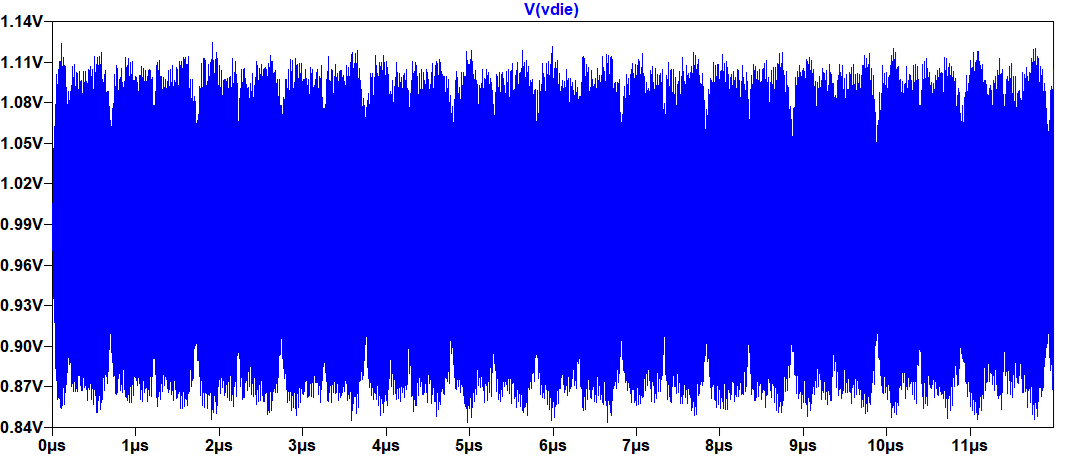
\includegraphics[width=\textwidth]{./eser4/vdie_time.png}
  \caption{Voltage at the die interface without decoupling capacitors over the whole simulation (12~$\mu$s).}
  \label{fig:vdie_time}
\end{figure}

\begin{table}[h]
  \centering
  \begin{tabular}{|l|c|}
    \hline
    \textbf{Quantity} & \textbf{Value} (full) \\
    \hline
    Peak-to-peak ripple (LTspice \texttt{.meas}) & 280.8~mV  \\
    Minimum voltage                              & 0.844~V   \\
    Maximum voltage                              & 1.125~V   \\
    Average voltage                              & 0.986~V   \\
    \hline
  \end{tabular}
  \caption{Voltage ripple at the die interface without decoupling capacitors.}
  \label{tab:ripple}
\end{table}

\noindent The ripple is really large: 281~mV peak-to-peak, which is 28\% of the supply voltage. The minimum is 0.844~V and the maximum is
1.125~V, so the voltage goes well outside a typical $\pm 5\%$ tolerance band, and this happens over the whole simulation, not only in a few
points. One could expect mainly a voltage drop, but the voltage actually goes both below and above 1~V, almost symmetrically. The average value
is 0.986~V: the 14~mV of difference from 1~V, with an average current of 109~mA, is the static drop on the DC resistance of the PDN.

\noindent\\ \autoref{fig:vdie_zoom} shows a zoom of 100~ns around the minimum of the voltage. Here the voltage looks almost like a sinusoid with a period of
10~ns, i.e.\ at 100~MHz, the same frequency of the activity of the die. The voltage does not follow each current pulse separately: the
oscillation grows over several cycles, which is the typical behaviour of a resonant circuit excited at its resonance frequency.

% FIGURE 2 - LTspice: same plot as Figure 1, click on the numbers of the time axis and set
% Left = 4.9u, Right = 5u (Y axis can stay 0.8-1.2 V). Export as latex/eser4/vdie_zoom.png
\begin{figure}[h]
  \centering
  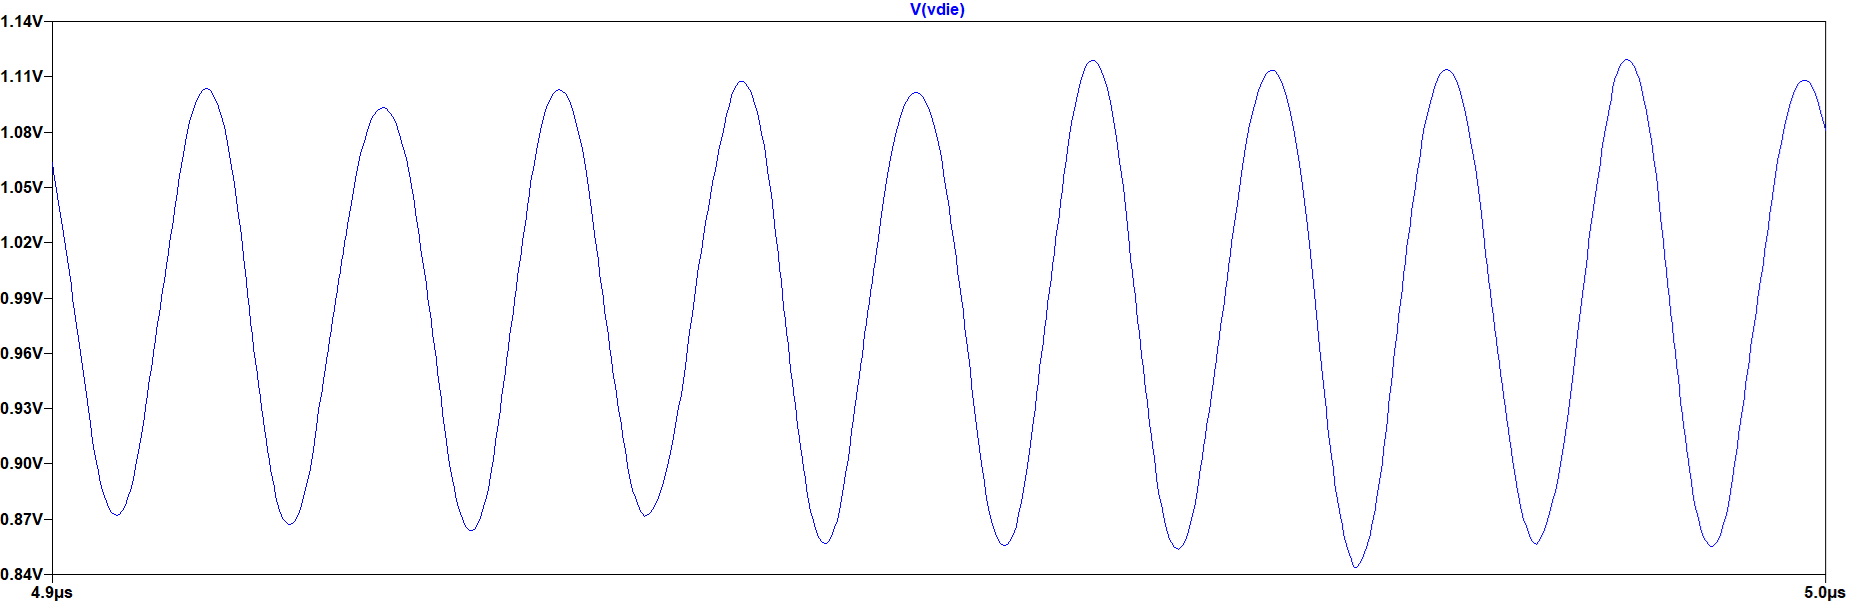
\includegraphics[width=\textwidth]{./eser4/vdie_zoom.png}
  \caption{Zoom of the voltage at the die interface over 100~ns, around the minimum of the voltage.}
  \label{fig:vdie_zoom}
\end{figure}



\noindent This is consistent with the result of Exercise~2: the impedance of the PDN
seen from the die has its main peak at about 96~MHz ($3.06~\Omega$), and at
100~MHz, the frequency of the main component of the die current, it is
still about $2.0~\Omega$.
The peak-to-peak ripple obtained in this work, about 281~mV, is higher than
the reference value of about 250~mV provided. This
difference is consistent with the result of Exercise~2: the maximum of the
PDN impedance obtained here is about $3.06~\Omega$, while the reference
value is about $2.9~\Omega$. Since the ripple is mainly caused by the die
current at the resonance of the PDN, a higher impedance peak produces a
proportionally higher ripple: both values are about 10\% higher
than the reference ones. The ripple is also confirmed by the
frequency-domain method of Exercise~5, which gives 282.2~mV without
decoupling capacitors.
So the problem is not the current itself, but the fact that its main component falls exactly on the resonance peak of the PDN. This also shows
what the decoupling capacitors have to do in Exercise~5: reduce the impedance at 100~MHz, or move the resonance away from the main frequency of the
die current.